\chapter{Componente hardware}
\label{chapter:hardware}

Hardware-ul reprezintă partea fizica a unui sistem informatic constituită din
diverse componente mecanice, electronice și optice. Cu ajutorul hardware-ului
se pot primi, prelucra și stoca informații. Și mai generic, prin hardware
înțelegem orice componentă într-un sistem complex de calcul ce poate fi atinsă,
există fizic într-o locație (pornind de la monitor, tastatură până la
componentele de comunicație, imprimante, etc.). Prin comparație, software-ul
este partea logică ce controlează diverse module din hardware pentru a îndeplini
sarcinile utilizatorului.

Într-o lume predominantă a software-ului, cuantificată prin numărul semnificativ
mai mare de companii care fac dezvoltare, prin numărul de angajați, numărul de
start-up-uri ce apar în fiecare an în comparație cu cele de hardware,
cunoașterea elementelor de hardware este esențială întrucât programele
dezvoltate trebuie să lucreze cu acestea. Din perspectiva utilizatorului,
cunoașterea componentelor hardware este esențială din mai multe perspective:
achiziție, instalare sistem de operare compatibil, instalare drivere
compatibile, optimizare rulare aplicații, depanare când apar probleme cu
sistemul.

La achiziția unui sistem de calcul (hardware-ul aferent practic), utilizatorul
trebuie să reușească să identifice caracteristicile cele mai bune pentru bugetul
dat. În general, nu e suficient să cunoască cele mai bune opțiuni deoarece
acestea sunt, adesea, cele mai scumpe și deseori nu se încadrează în bugetul
utilizatorilor. Cunoașterea componentelor hardware, tipul și prețul lor,
compatibilitatea între acestea, ajută la achiziția unui sistem de calcul cu cel
mai bun raport preț/calitate.

După achiziție urmează, în general, instalarea unui sistem de operare (dacă
sistemul de calcul nu a venit cu unul preinstalat - dar chiar și atunci se
dorește personalizarea lui). Pentru alegerea unui sistem de operare
corespunzător, trebuie cunoscute caracteristicile componentelor hardware
(arhitectura, memorie, dispozitive auxiliare), iar pentru buna funcționare a
tuturor extensiilor hardware (plăci grafice, camere video) este necesară
instalarea unui software specializat numit driver. Alegerea driver-ului este
foarte importantă și este strict legată de tipul dispozitivului fizic, precum și
modelul acestuia. Alegerea unui driver necorespunzător nu va permite folosirea
dispozitivului fizic la parametri normali sau chiar deloc, iar în cel mai rău
caz poate cauza probleme cu stabilitatea sistemului (acele blue-screen-uri pe
Windows, reset-uri spontane, etc).

În următoarele secțiuni vom realiza o clasificare a sistemelor de calcul
(hardware) în funcție de diverse criterii (arhitecturi, dimensiuni fizice, forme
de împachetare a componentelor) și vom descrie interacțiunea dintre
dispozitivele hardware și sistemele de operare. Spre finalul capitolului vom
prezenta rolul extensiilor auxiliare (plăci) și facilități moderne incluse în
hardware-ul din ziua de astăzi. Capitolul se încheie cu două studii de caz
legate de vizualizare componentelor hardware și a versiunilor de driver pe două
sisteme de operare de uz general: Linux și Windows.

\section{Clasificarea sistemelor de calcul (hardware-ului)}
\label{sec:hardware-class}

Rolul acestui capitol este dat de prezentarea componentelor hardware cu scopul
de a putea alege un sistem de calcul, diagnostica o problema cu un sistem de
calcul și de a instala software-ul potrivit. Sistemul de calcul (sistemul
hardware) pentru a îndeplini sarcinile dorite de utilizator are nevoie de 3
componente principale: procesare (echivalentul creierului la om), stocare
(înmagazinarea datelor procesate pentru a fi accesate ulterior - echivalentul
unei cărți) și de un mecanism prin care să introducem și să preluăm date de la
componenta de procesare (în termeni tehnici acesta se numește subsistemul
intrare/ieșire sau I/O - de la input/output).

Un prim pas pentru îndeplinirea obiectivelor enunțate mai sus este dat de
definirea unor clasificări (tipuri) ale hardware-ului din mai multe perspective.
Vom porni de la o descriere logica a hardware-ului numită și \texttt{Arhitectura
von Neumann}. Numele arhitecturii provine de la matematicianul și fizicianul
John von Neumann care a scris primul draft al raportului EDVAC
\abbrev{EDVAC}{Electronic Discrete Variable Automatic Computer} în 1945 ce
descria arhitectura unui sistem de calcul.

%(https://sites.google.com/site/michaeldgodfrey/vonneumann/vnedvac.pdf?attredirects=0&d=1)

\subsection{Arhitectura von Neumann}
\label{sec:hardware-class-neumann}

Arhitectura von Neumann reprezintă o descriere logică a unui sistem de calcul ce
enumeră următoarele tipuri de componente:

\begin{itemize}
	\item Unitate de procesare / Procesor (Central Processing Unit - CPU
		\abbrev{CPU}{Central Processing Unit})
	\item Unitate de memorie (Memory Unit - \abbrev{MU}{Memorty Unit})
	\item Dispozitive de intrare/ieșire (Input-Output - I/O)
\end{itemize}

In \labelindexref{Figura}{fig:hw-neumann} este reprezentată grafic această
arhitectură. Unitatea de procesare este formată din unitatea de control și
unitatea aritmetică/logică. Unitatea de control are rolul de a configura și a da
comenzi perifericelor, respectiv unității aritmetice/logice, pentru a
întreprinde acțiunile dorite de utilizator. Unitatea aritmetică/logică se ocupă
în general cu realizarea calculelor, fiind optimizată pentru acest lucru.
Aceasta are un rol foarte important deoarece majoritatea comenzilor
utilizatorului se vor traduce în final către hardware în operații de aritmetică
(ex. adunare) sau de logică (și/sau/xor). Unitatea de memorie are rolul de a
servi rapid procesorul cu datele necesare realizării calculelor. Datele în
general vin de la utilizator prin dispozitivele de intrare și sunt stocate
temporar de unitatea de memorie pentru a putea fi folosite de unitatea de
procesare. Acest flux a fost creat din cauza faptului ca dispozitivele
periferice (intrare/ieșire) sunt mult mai lente în general decât unitatea de
procesare și ar încetini-o. Unitatea de memorie în general este volatilă (la
închiderea sistemului, datele din unitatea de memorie se pierd) fiind folosită
ca un tampon pentru prelucrarea datelor. Odată prelucrate, acestea sunt trimise
către dispozitivele de ieșire și folosite în diverse scopuri (afișare, stocare
permanentă).

\begin{figure}[!htbp]
	\centering
	\def\svgwidth{\columnwidth}
	\includesvg{chapters/08-hw/img/arch-neumann.svg}
	\caption{Arhitectura von Neumann}
	\label{fig:hw-neumann}
\end{figure}

În zilele noastre numărul unităților de procesare a crescut, precum și mărimea
unității de memorie. Unitatea de memorie este partajată între toate
procesoarele folosind o singură legătură între acestea denumită magistrală.
Acest lucru s-a dovedit a fi un punct de congestie pentru procesoare întrucât
acestea așteaptă fiecare pentru magistrală. Pentru optimizare, în implementările
curente s-au introdus memorii specifice fiecărui procesor numite cache. Un alt
motiv pentru introducerea memoriei cache a fost dată și de faptul că memoria
principală este cu câteva ordine de mărime mai înceată decât unitatea de
procesare. O altă optimizare, în afară de memoria cache, a fost reprezentată de
arhitectura Harvard unde s-a separat memoria de instrucțiuni (control) de
memoria de date (intrare). Cu toate aceste optimizări, fiecare sistem calcul
respectă arhitectura logică von Neumann, indiferent de tehnologia folosită și
modul de integrare a componentelor.

În limbajul comun (de zi cu zi) folosim noțiunea de \textit{procesor} pentru
unitatea de calcul, \textit{memorie} pentru unitatea de memorie, \textit{I/O}
pentru dispozitivele de intrare sau ieșire. \textit{Disc/hard} reprezintă un
dispozitiv I/O pentru stocarea permanentă a datelor, iar \textit{placa de rețea}
este și ea un dispozitiv I/O pentru comunicarea între diferite unități de
calcul.

\subsection{Arhitecturi de procesor}
\label{sec:hardware-class-proc}

În zilele noastre dispozitivele hardware folosesc procesoare (unități de calcul)
de la diverși producători. Aceste procesoare respectă în general două
arhitecturi cunoscute: x86 și ARM. x86 este folosit în general în sistemele
desktop, laptop-uri, servere, iar arhitectura ARM este folosită în general în
dispozitivele mobile (smarthphone-uri, tablete).

Pornind de la modelul von Neumann prezentat anterior, putem realiza o
clasificare a unității de procesare în funcție de tipul instrucțiunilor pe care
îl execută (se mai numește și set de instrucțiuni sau arhitectura sistemului,
prescurtat deseori ISA \abbrev{ISA}{Instruction Set Architecture}, Instruction
Set Architecture).

Astfel, în zilele noastre, sistemele de calcul respectă una din următoarele 2
arhitecturi:

\begin{itemize}
	\item Reduced instruction set computer (referită de acum încolo prin
		acronimul RISC \abbrev{RISC}{Reduce Instruction Set Computer})
	\item Complex instruction set computer (referită de acum încolo prin
		acronimul CISC \abbrev{CISC}{Complex Instruction Set Computer})
\end{itemize}

Înainte de a defini arhitecturile RISC/CISC vom mai introduce câteva elemente
componente ale unității de procesare. Execuția instrucțiunilor se realizează
asupra unor operanzi. Acești operanzi ar putea fi locații de memorie, dar acest
lucru ar încetini unitatea de calcul la viteza de acces a datelor din memorie.
Pentru a preveni accesul lent la date, au fost introduse registrele. Registrele
sunt la baza memorii foarte rapide, de dimensiune fixă, dată de arhitectura
constructivă a unității de procesare (32biți/64biți - cele mai frecvente în ziua
de astăzi sunt arhitecturile pe 64 de biți). Instrucțiunile au în general zero
sau mai mulți operanzi referiți prin registre. Inclusiv locațiile de memorie
asupra cărora se fac modificări sunt referite tot prin registre (se încarcă
adresa memoriei în registru iar acesta este folosit în execuția instrucțiunii).

Arhitectura de tip RISC este cunoscută și sub numele de arhitectură
\textit{load/store}:
orice operație (de adunare, scădere) se realizează prin încărcarea conținutului
memoriei în registre (load), iar după finalizarea operației conținutul
registrelor este salvat în memorie (store). Instrucțiunile nu pot referi în mod
direct memoria.

Arhitectura de tip CISC poate executa în aceeași instrucțiune primită de la
utilizator mai multe operații numite micro-instrucțiuni: dacă dorim să adunăm
două numere din memorie, putem executa o singură instrucțiune care va referi
cele 2 locații de memorie; în spate instrucțiunea este tradusă în mai multe
micro-instrucțiuni (încărcare operanzi în registre, adunare, salvare rezultate);
pentru acest exemplu avem o singură instrucțiuni dată de utilizator pentru
arhitectura CISC, iar pentru arhitectura RISC vom avea 3 instrucțiuni specifice
diferite.

Pentru ambele tipuri de arhitecturi există avantaje și dezavantaje. La RISC
arhitectura internă este mult mai simplă, dar trebuie generate mai multe
instrucțiuni pentru o operație, iar la CISC arhitectura internă este mai
complexă, predispusă bug-urilor, dar într-o singură instrucțiune se pot
îndeplini mai multe sarcini. O să observăm în continuare că avem exemple în
producție din ambele tipuri, fiecare specific unui anumit domeniu.

În afară de clasificarea legată de setul de instrucțiuni (ISA - RISC vs CISC),
se mai poate realiza o clasificare legată de dimensiunea adresării memoriei:
câți biți sunt folosiți pentru a adresa o locație de memorie. În legătură
directă cu dimensiunea adresării se află și dimensiunea registrelor întrucât
acestea sunt folosite pentru a realiza adresarea. În zilele noastre avem în
general 2 tipuri de adresări:

\begin{itemize}
	\item Pe 32 de biți din ce în ce mai puțin folosită, dar păstrată din
		motive de compatibilitate
	\item Pe 64 de biți folosită preponderent în ziua de astăzi inclusiv în
		piața de mobile
\end{itemize}

Trecerea de la 32 de biți la 64 de biți s-a realizat atunci când dimensiunea
memoriei a crescut mai mult de patru gigaocteți (gigabytes). Folosind 32 biți
putem itera prin adrese de la 0 la 4 gigaocteți ($2^{32}$). Pentru a rezolva
acest deficit s-a trecut la o arhitectură pe 64 de biți ce poate adresa
semnificativ mai mult ($2^{64}$ teoretic, $2^{48}$ în practică din cauza
limitărilor hardware cum ar fi folosirea unui număr mai mic de tranzistori).

\subsection{Arhitectura x86 și arhitectura ARM}
\label{sec:hardware-class-arm-x86}

În zilele noastre există două mari arhitecturi:

\begin{itemize}
	\item x86 - disponibil atât pe 32 de biți (referit ca x86), cât și pe 64
		de biți (referit ca x86_64 sau x64), fiind o arhitectură de tip
		CISC. Un exemplu este reprezentat în
		\labelindexref{Figura}{fig:hw-x86} un calculator ce are o
		arhitectura x86

\begin{figure}[!htbp]
	\centering
	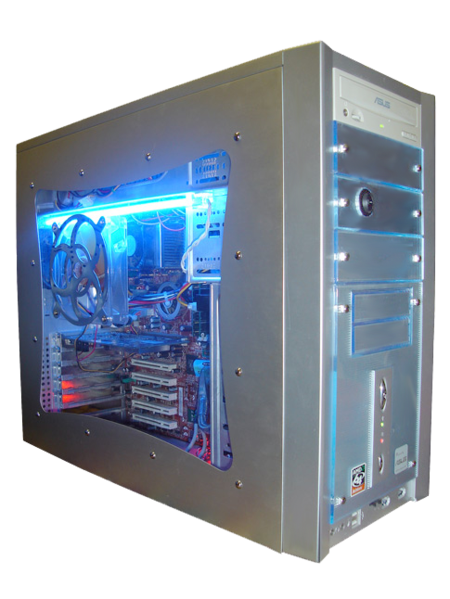
\includegraphics[width=4cm]{chapters/08-hw/img/pc-img.png}
	\caption{Calculator cu arhitectura x86\protect\footnotemark}
	\label{fig:hw-x86}
\end{figure}

\footnotetext{https://commons.wikimedia.org/wiki/File:Modified-pc-case.png
\textbf{CC BY SA}}

	\item ARM - disponibil atât pe 32 de biți (referit ca ARMv7), câț și pe
		64 de biți (referit ca ARMv8), fiind o arhitectură de tip RISC.
		Un exemplu este reprezentat în
		\labelindexref{Figura}{fig:hw-arm} un smartphone cu arhitectura
		ARM. După cum se poate observa toate componentele sunt integrate
		pe aceeași plăcută în comparație cu arhitectura x86.

\begin{figure}[!htbp]
	\centering
	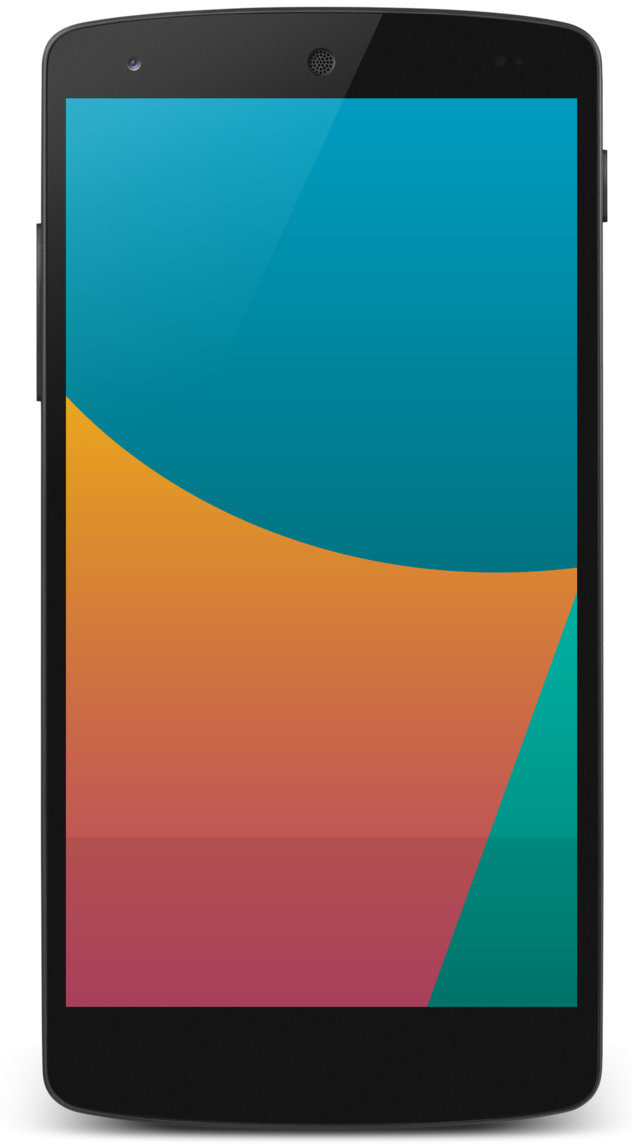
\includegraphics[width=4cm]{chapters/08-hw/img/arm-img.png}
	\caption{Smartphone cu arhitectura ARM\protect\footnotemark}
	\label{fig:hw-arm}
\end{figure}

\footnotetext{\url{https://en.wikipedia.org/wiki/Nexus_5\#/media/File:Nexus_5_Front_View.png}
\textbf{CC BY 2.5}}

\end{itemize}

Pentru arhitectura x86 există 2 producători care împart procentele din piață:
Intel și AMD (aceștia proiectează și implementează hardware-ul). Arhitectura ARM
are un alt model de dezvoltare: compania ARM vinde proiectele procesorului către
producătorii interesați, iar aceștia le integrează cu alte componente periferice
și le implementează (exemplu Apple și Samsung).

Arhitectura x86 este folosită cu precădere în sisteme de tip desktop, laptop și
server. Pentru fiecare tip de sistem, există versiuni diferite de procesor:

\begin{itemize}
	\item Pentru desktop avem procesoare pretabile aplicațiilor de zi cu zi
	\item Pentru laptop avem procesoare ce respectă caracteristicile unui
		sistem desktop, dar dispun de un consum redus de energie
	\item Pentru servere avem procesoare cu un număr mare de unități de
		procesare (sau core-uri în limbaj tehnic), cache-uri mai mari,
		răcire eficientă
\end{itemize}

Arhitectura ARM este folosită cu precădere în dispozitivele embedded/mobile.
Majoritatea telefoanelor smart din ziua de astăzi au un procesor ARM (cei mai
mari vendori fiind Apple și Samsung). În cadrul telefoanelor smart există 2
tipuri de procesoare: pe 32 de biți (majoritatea) și pe 64 de biți. Procesoarele
ARMv7 au o adresare pe 32 de biți, iar procesoarele ARMv8 au o adresare pe 64 de
biți. Avantajul ARM în fața x86 este consumul redus de energie și numărul
ridicat de core-uri pe care îl poate oferi. La momentul scrierii ARM are
intenția de a intra pe piața serverelor concurând cu Intel și AMD. Există
diverse prototipuri folosind procesoare ARMv8 ce ating performanțele
procesoarelor Intel, la un cost redus. De asemenea, Intel a încercat folosirea
procesoarelor x86 în telefoanele mobile smart, dar nu au reușit să creeze un
produs stabil și să câștige o cotă de piață relevantă, fiind că sunt mereu în
urma procesoarelor ARM cu 1-2 ani. În acest moment, Intel a renunțat să mai
investească în acest segment.

O altă diferență între cele 2 arhitecturi (x86 și ARM) o reprezintă modelul de
integrare a componentelor:

\begin{itemize}
	\item x86 are o arhitectură modulară în care utilizatorul poate înlocui
		separat procesorul, memoria, plăcile de procesare (grafică,
		sunet, rețea)
	\item ARM are o arhitectură integrată denumită și SoC (System on Chip):
		integratorii pun toate componentele (procesorul, memoria,
		plăcile de procesare) pe aceeași plăcuță iar acestea nu pot fi
		schimbate separat
	\item rme constructive ale hardware-ului
	\item stemele de calcul vin în diverse forme constructive (form factors
		- dimensiune, forma de împachetare a componentelor) în funcție
		rolul și utilizarea acestora. Într-o clasificare generică avem
		patru forme constructive:
	\item Server - specific centrelor de date
	\item Desktop - specific utilizatorilor obișnuiți
	\item Laptop - specific utilizatorilor finali, ocupând mai puțin spațiu
		și având un cost mai mare ca sistemele Desktop în general
	\item Embedded - specific dispozitivelor mobile (smartphone-uri /
		tablete) și industriale
\end{itemize}

\textit{Serverul} este specific centrelor de date având o construcție robustă,
sisteme de prindere speciale în locurile special amenajate, o circulație a
aerului pe orizontală foarte bună (în general din față în spate). Dimensiunea
serverelor este dată de numărul unităților de rack ocupate (1U = \texttt{4,445cm}). In
\labelindexref{Figura}{fig:hw-server} este ilustrat un server de dimensiune 1U
(1 unitate de rack), cu sisteme de prindere în lateral. După cum se poate
observa aerul va circula din față în spate și niciodată pe deasupra sau dedesubt
din cauza modului în care serverele sunt așezate în rack: unul peste altul fară
nici un spațiu.

\begin{figure}[!htbp]
	\centering
	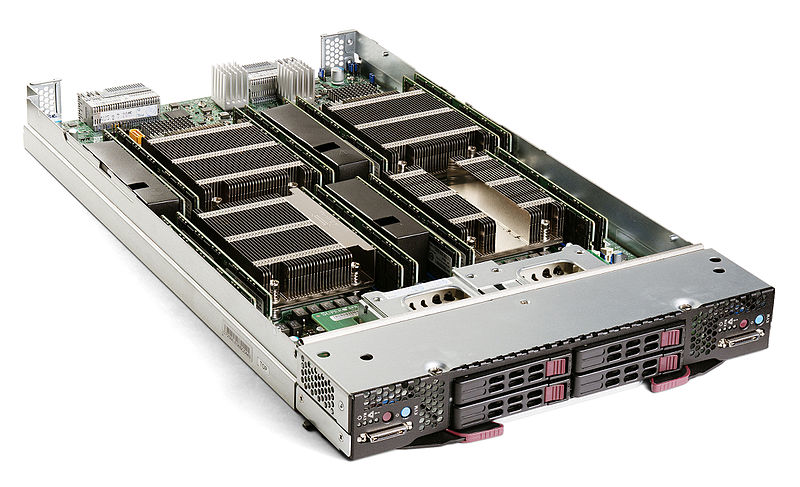
\includegraphics[width=6cm]{chapters/08-hw/img/server-img.png}
	\caption{Server\protect\footnotemark}
	\label{fig:hw-server}
\end{figure}

\footnotetext{\url{https://commons.wikimedia.org/wiki/File:Supermicro_SBI-7228R-T2X_blade_server.jpg}
\textbf{CC BY SA 4.0}}

\textit{Desktop}-ul este specific utilizatorilor finali având un raport
preț/performanță foarte bun. După cum am precizat mai sus, laptop-ul tot
utilizatorului final se adresează. Avantajul desktop-ului în detrimentul
laptop-ului este dat de faptul că poate fi ușor îmbunătățit, reparat și
întreținut.

Desktop-ul vine și el în mai multe forme constructive:

\begin{itemize}
	\item Small factor
	\item Normal factor
\end{itemize}

\textit{Small factor} se referă la o carcasă compactă de mici dimensiuni ce
poate fi pusă inclusiv pe birou, iar normal factor este o carcasa de dimensiuni
mai mari. Avantajul small factor este după cum am precizat anterior
dimensiunea redusă, iar dezavantajul este dat de faptul că suportă un număr
limitat de extensii auxiliare (în general nu este loc și pentru ele în carcasă).
Dezavantajul normal factor este dat de dimensiune, dar este mult mai ușor de
personalizat.

\begin{figure}[!htbp]
	\centering
	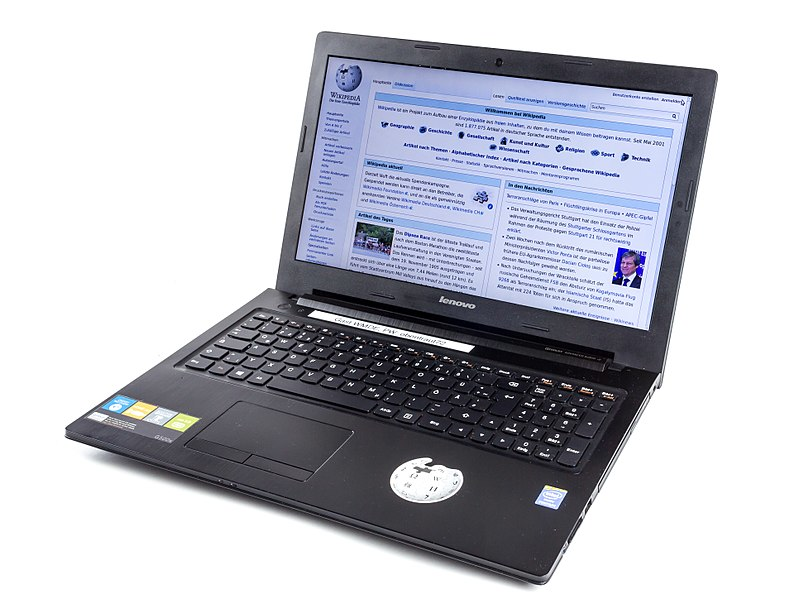
\includegraphics[width=6cm]{chapters/08-hw/img/laptop-img.png}
	\caption{Laptop\protect\footnotemark}
	\label{fig:hw-laptop}
\end{figure}

\footnotetext{\url{https://commons.wikimedia.org/wiki/File:Lenovo_G500s_laptop-2905.jpg}
\textbf{CC BY-SA 4.0}}

\textit{Laptop-urile} reprezintă un alt model constructiv al unui calculator
pentru a adresa portabilitatea (vezi \labelindexref{Figura}{fig:hw-laptop}). De
obicei acestea conțin din fabrică toate componentele dorite și este mai dificil
de personalizat (în general se poate adăuga mai multă memorie, se poate schimba
unitatea de stocare, dar cam atât).

\textit{Sistemele embedded} (vezi \labelindexref{Capitolul}{chapter:embed}), de obicei,
nu au o carcasă cu care vin de la producător. Acestea sunt niște plăcuțe care
conțin toate perifericele integrate (SoC - System on Chip).
\labelindexref{Figura}{fig:hw-embed} prezintă un astfel de sistem embedded
(integrat).

\begin{figure}[!htbp]
	\centering
	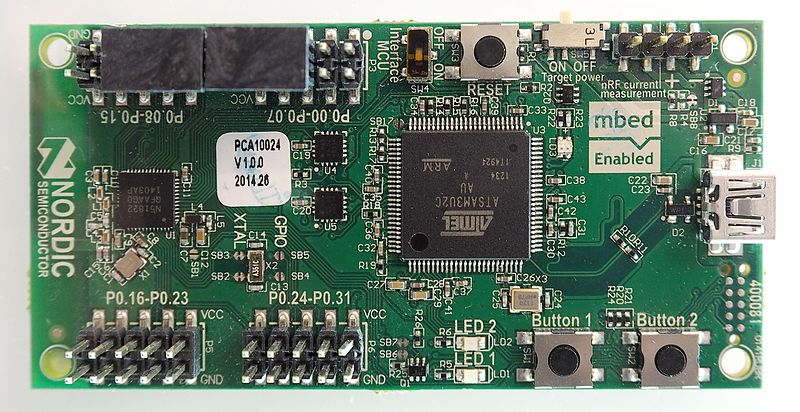
\includegraphics[width=7cm]{chapters/08-hw/img/embedded-img.png}
	\caption{Sistem embedded (integrat)\protect\footnotemark}
	\label{fig:hw-embed}
\end{figure}

\footnotetext{\url{https://commons.wikimedia.org/wiki/File:Embedded_World_2016,_Nordic_RF51822.jpg}
\textbf{CC0}}

\section{Componentele unui sistem de tip desktop}
\label{sec:hardware-componente}

În capitolul anterior s-au prezentat diferite forme constructive ale unui sistem
de calcul. În acest capitol vom descrie componența unui sistem de tip desktop.
Această componență este valabilă și pentru celelalte forme constructive ale
sistemelor de calcul (server, laptop, embedded) doar că sunt dispuse și
integrate în poziții diferite.

\begin{figure}[!htbp]
	\centering
	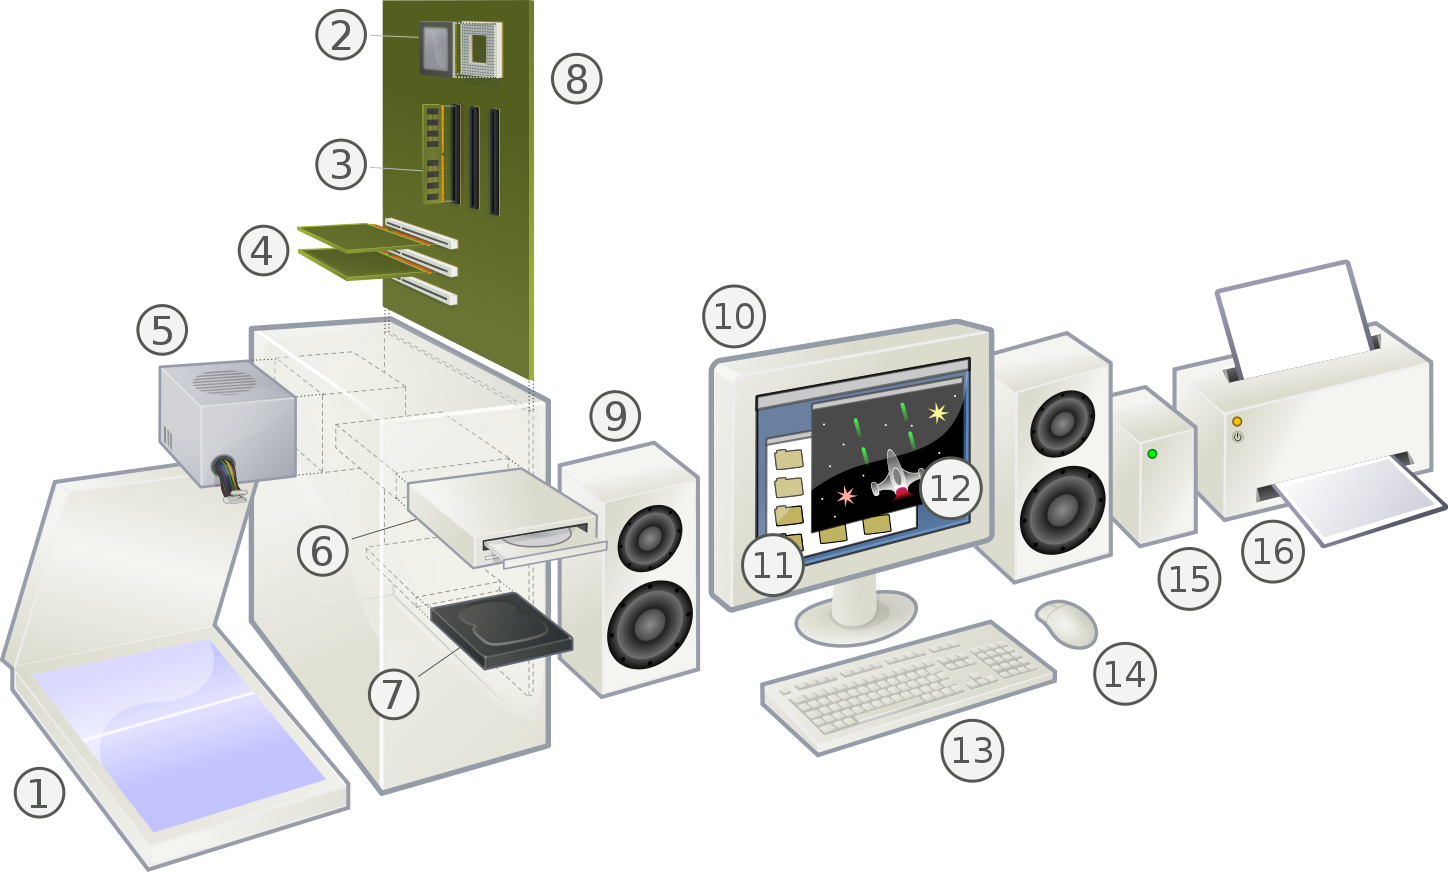
\includegraphics[width=8cm]{chapters/08-hw/img/comps-img.png}
	\caption{Componentele unui calculator\protect\footnotemark}
	\label{fig:hw-comps}
\end{figure}

\footnotetext{\url{https://commons.wikimedia.org/w/index.php?curid=4023664}
\textbf{CC BY 2.5}}

\begin{enumerate}
	\item Scanner - cu ajutorul acesteia se pozează conținutul documentelor
		cu scopul de la fi digitalizate (transferate pe calculator).
		Acesta este un dispozitiv de intrare
	\item CPU - procesorul (unitatea de procesare) execută instrucțiunile
		primite de la utilizator. Principalele caracteristici sunt
		frecvența (în mega/giga herți - Mhz/Ghz) care determină numărul
		de instrucțiuni executate pe secundă, mărimea memoriei cache,
		numărul de nuclee (un CPU poate avea mai multe unități de
		execuție înglobate în aceeași pastilă) și viteza cu care
		comunică cu restul componentelor prin intermediul magistralei
		(se mai numește și frecvența magistralei [FSB
		\abbrev{FSB}{Front-Side Bus}]).

\begin{figure}[!htbp]
	\centering
	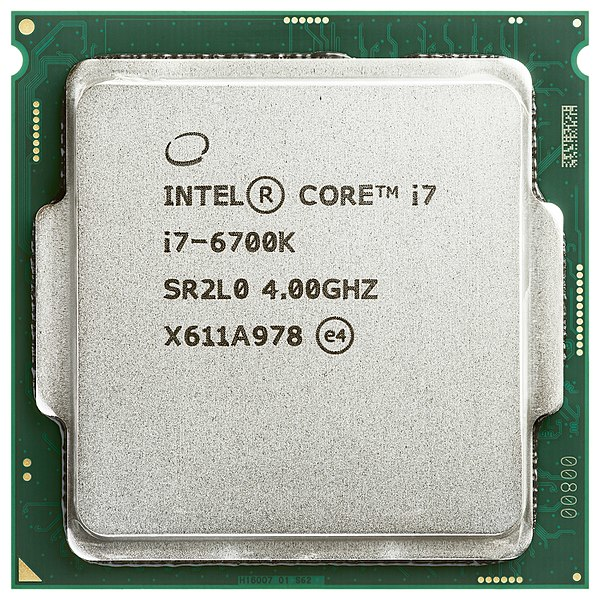
\includegraphics[width=7cm]{chapters/08-hw/img/cpu-img.png}
	\caption{CPU (procesorul)\protect\footnotemark}
	\label{fig:hw-cpu}
\end{figure}

\footnotetext{\url{https://commons.wikimedia.org/wiki/File:Intel_CPU_Core_i7_6700K_Skylake_top.jpg}
\textbf{CC BY SA}}

	\item Memoria - unitatea de memorie care este de tip RAM
		\abbrev{RAM}{Random Access Memory} (Random Access Memory) și
		este reprezentată de o plăcuță îngustă care poate avea diferite
		dimensiuni exprimate în megaocteți (MB \abbrev{MB}{megabytes} -
		megabytes) sau gigaocteți (GB \abbrev{GB}{gigabytes} -
		gigabytes). O altă caracteristică a memorie se referă la
		frecvența acesteia în general exprimată în megaherți (MHz
		\abbrev{MHz}{megaherți}). Frecvența reprezintă viteza cu care
		se realizează comunicația între memorie și magistrală, respectiv
		procesor.

\begin{figure}[!htbp]
	\centering
	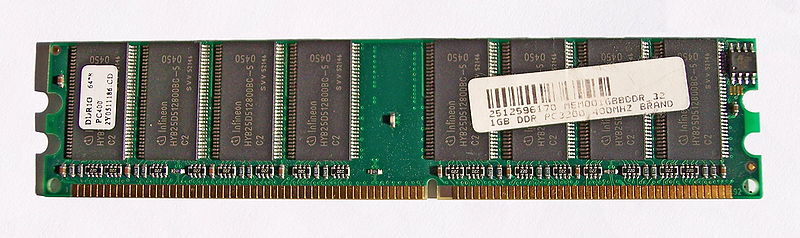
\includegraphics[width=8cm]{chapters/08-hw/img/ram-img.png}
	\caption{Memoria RAM\protect\footnotemark}
	\label{fig:hw-ram}
\end{figure}

\footnotetext{\url{https://commons.wikimedia.org/wiki/File:DDR_RAM-3.jpg}
\textbf{Public domain}}

	\item Plăci de extensie: acestea sunt variante pornind de la plăcile de
		procesare a sunetului (pentru redarea acestuia), a elementelor
		grafice (pentru afișarea pe ecran) până la plăcile ce realizează
		conectivitatea cu alte calculatoare (respectiv Internetul). Vom
		extinde subiectul plăcilor de extensie în secțiunile următoare
	\item Sursa de alimentare a unității de calcul: transforma curentul
		alternativ în curent continuu la diferite voltaje/intensități
		pentru fiecare componentă a sistemului de calcul. Principala
		caracteristică a surselor de alimentare este data de putere
		(watt). Sursa trebuie sa fie dimensionată corespunzător pentru a
		reuși să acopere toți consumatorii din sistem (ex.: dacă avem un
		procesor mai puternic, cu o frecvență mai mare și mai multe
		nuclee avem nevoie de o sursă de putere mai mare)
	\item Unitate optică (CD/DVD - ROM \abbrev{ROM}{Read-Only Memory}) -
		acesta este un dispozitiv de intrare/ieșire persistent pentru
		redarea filmelor, a muzicii, dar se pot stoca și date care nu au
		legătură cu aria multimedia (ex.: documente)

\begin{figure}[!htbp]
	\centering
	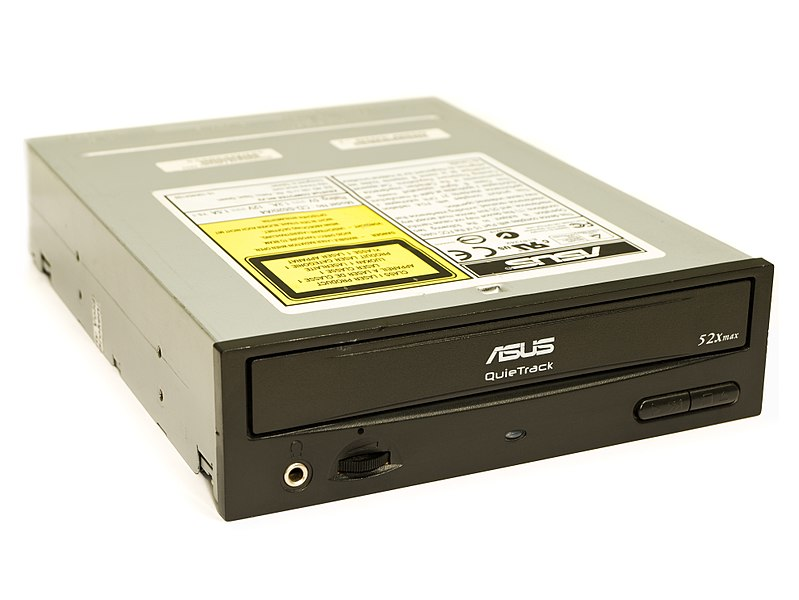
\includegraphics[width=8cm]{chapters/08-hw/img/dvd-img.png}
	\caption{DVD-ROM\protect\footnotemark}
	\label{fig:hw-dvd}
\end{figure}

\footnotetext{\url{https://commons.wikimedia.org/wiki/File:ASUS_CD-ROM_CD-S520-A4_20080821.jpg}
\textbf{CC BY 3.0}}

	\item Unitate de stocare (HDD \abbrev{HDD}{Hard Disk Drive} - Hard Disk
		Drive) - acesta este un dispozitiv de intrare/ieșire pentru
		stocarea permanentă/persistentă a datelor. De exemplu, ori de
		câte ori salvăm un fișier în curs de editare, acesta este scris
		pe unitatea de stocare. Aceasta este mult mai lentă ca unitatea
		de memorie și de aceea se preferă scrierea cât mai rară, în
		special când se întreprind acțiuni în timp real.

\begin{figure}[!htbp]
	\centering
	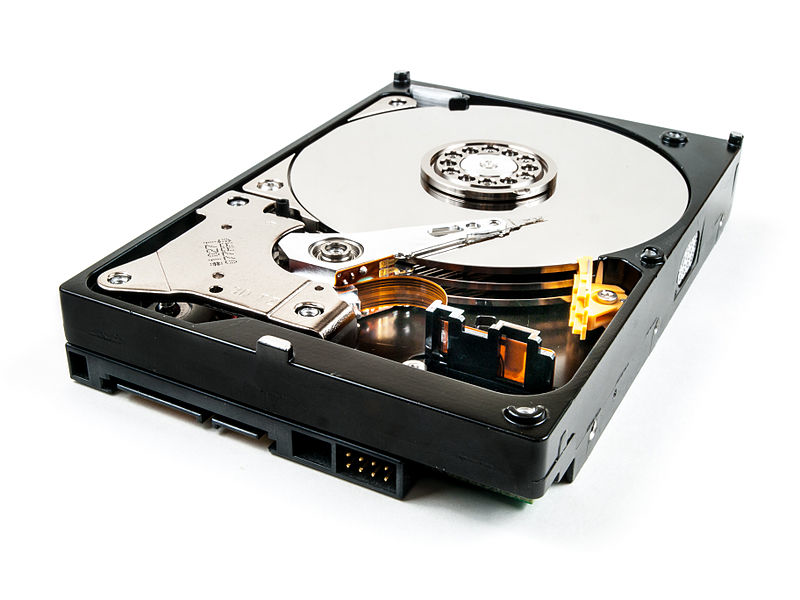
\includegraphics[width=8cm]{chapters/08-hw/img/hdd-img.png}
	\caption{Discul pentru stocare - HDD\protect\footnotemark}
	\label{fig:hw-hdd}
\end{figure}

\footnotetext{\url{https://commons.wikimedia.org/wiki/File:Hard_Drive_(11644419853).jpg}
\textbf{CC BY 2.0}}

	\item Placa de bază reprezintă elementul central de conexiune între
		procesor, memorie și plăcile de extensie. Aceasta conține
		practic magistrala de comunicație și sloturile în care sunt
		introduse procesorul, memoriile și plăcile de extensie.

% TODO: this doesn't fit
%\begin{figure}[!htbp]
%	\centering
%	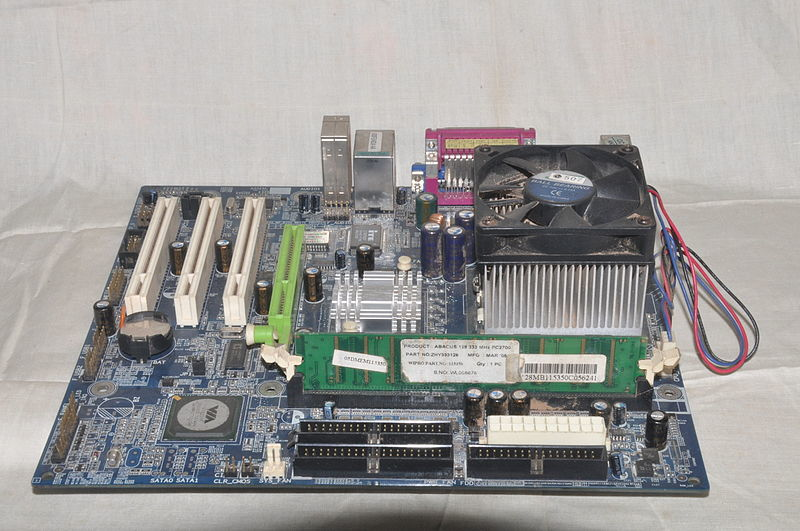
\includegraphics[width=8cm]{chapters/08-hw/img/mb-img.png}
%	\caption{Placa de bază\protect\footnotemark}
%	\label{fig:hw-mb}
%\end{figure}

%\footnotetext{\url{https://commons.wikimedia.org/wiki/File:Mother_board.JPG}
%\textbf{CC BY SA 4.0}}

	\item Boxe conectate la placa de extensie (numită și placă de sunet)
		pentru a reda sunetul emis de unitatea de calcul
	\item Monitorul conectat la placa de extensie (numită și placă grafică
		sau GPU \abbrev{GPU}{Graphics Processing Unit} în acest caz)
		pentru a reda elementele grafice.
	\item Sistemul de operare - software-ul ce este responsabil cu
		inițializarea și controlul componentelor hardware
	\item O aplicație (joculeț) ce rulează în sistemul de operare
	\item Tastatură - dispozitiv de intrare prin care utilizatorul trimite
		comenzi către calculator sau poate redacta diverse documente
	\item Mouse - dispozitiv de intrare pentru a ușura controlul sistemului
		de operare și a aplicațiilor (care este posibil prin intermediul
		tastaturii, dar în medii grafice, operarea doar din tastatură
		devine foarte greoaie)
	\item Unitate de stocare externă (HDD extern - portabil) - acesta are
		același rol ca și Unitatea de stocare prezentată la punctul 7,
		cu avantajul de a fi portabilă și dezavantajul că este de obicei
		mai lent.

\end{enumerate}

Acestea sunt elementele de bază ale unui sistem de calcul din zilele noastre. În
mod curent există diverse extensii, dispozitive specializate ce se conectează la
calculator (stick USB pentru comunicații, pentru stocare, token pentru
criptare), dar folosesc aceleași interfețe ca unul din dispozitivele de mai sus.

\section{Interacțiunea hardware - sistem de operare}
\label{sec:hardware-interact}

Până la această secțiune am prezentat arhitectura logică a unui sistem de
calcul, am enumerat clasificări în funcție de mai multe criterii (arhitectura
unității de procesare, forma constructivă a sistemului de calcul), am iterat
principalele componente ale unui sistem de tip desktop. Toate acestea trebuie
controlate de un software specializat care poartă numele de sistem de operare.
Sistemul de operare (OS - acronim folosit în industrie) este primul program
(software) ce rulează la pornirea unui sistem de calcul. Rolurile sistemul de
operare sunt următoarele:

\begin{itemize}
	\item Descoperirea dispozitivelor ce formează sistemul de calcul
	\item Inițializarea și configurarea dispozitivelor
	\item Controlul dispozitivelor
\end{itemize}

Vom discuta despre descoperirea dispozitivelor în contextul celor două
arhitecturi folosite în sistemele de uz general din ziua de astăzi (x86 și ARM).
Descoperirea dispozitivelor se face folosind următoarele procedee:

\begin{itemize}
	\item Autodiscovery (descoperire automată de către sistemul de operare)
		în general pe x86 - la pornirea sistemului rulează un program
		proprietar al plăcii de bază denumit BIOS \abbrev{BIOS}{Basic
		Input/Output System} (Basic Input/Output System - vezi
		\labelindexref{Capitolul}{chapter:boot}) care testează toate
		componentele conectate la placa de bază, certifică
		compatibilitatea acestora (între ele și cu placa de bază). Cel
		mai important lucru este dat de faptul ca încarcă sistemul de
		operare de pe disc în memorie și pornește execuția acestuia. Din
		acest punct sistemul de operare este cel care va face din nou
		descoperirea tuturor componentelor, inițializarea și
		configurarea, precum și controlul acestora. Totul este făcut
		automat prin scanarea și enumerarea unor locații speciale din
		memorie pentru a identifica fiecare componentă.
	\item DTB \abbrev{DTB}{Device Tree Blob} (Device Tree Blob) în general
		pe ARM - pe sistemele ARM în general nu există noțiunea de BIOS
		întrucât totul este integrat pe o singură plăcuță (SoC - System
		on Chip) și nu avem nici o configurație hardware dinamică (totul
		este prestabilit de la bun început). Aici există specificații
		clare la ce adresă trebuie încărcat sistemul de operare și de
		unde începe execuția acestuia. Fiind totul integrat într-un SoC,
		integrarea variind de la vendor la vendor (ex. adresa de început
		a memoriei este diferită), nu există nici un mecanism de
		Autodiscovery. În general producătorul oferă un DTB (Device Tree
		Blob) în care este descrisă fiecare componentă SoC-ului. Acest
		DTB este încărcat în memorie împreună cu sistemul de operare,
		iar acesta parsează acest DTB pentru a vedea de elemente are la
		dispozitie cu scopul de a le inițializa, configura și controla.
\end{itemize}

În ambele cazuri prezentate mai sus (Autodiscovery vs. DTB), până la rularea
sistemului de operare, în practică, mai există un nivel de software numit
\textit{boot loader}. Boot loader-ul este de fapt programul care rulează imediat
după BIOS, în cazul x86, și imediat după pornirea sistemului, în cazul ARM. Boot
loader-ul are rolul de a încărca sistemul de operare în memorie. În cazul x86
cel mai folosit boot loader pe sistemele Linux este GRUB, iar pe sistemele
Windows este unul proprietar. În cazul ARM avem un singur boot loader numit
U-BOOT. Mai multe detalii despre Boot loader, motivul pentru care acesta a fost
introdus, ce opțiuni de configurare oferă, se pot vedea în capitolul următor
(\textit{Pornirea sistemului}).

Un exemplu simplu, care apare proeminent în viața de zi cu zi este folosirea
unei imprimante. În general pentru a putea folosi imprimantă, spunem că aceasta
trebuie instalată. Mai specific, trebuie instalat un driver pentru aceasta.
Driverul este util sistemului de operare pentru putea controla dispozitivul (să
ii dea comenzi de printare în acest caz și să primească răspunsuri de la acesta
relativ la starea acțiunii de printare). Fără driver, dispozitivul nu ar putea
fi folosit.

O dată încărcat sistemul de operare, acesta este lansat în execuție. Din acest
punct se va începe descoperirea tuturor elementelor hardware (de la procesor,
memorie până la toate perifericele conectate), inițializarea și configurarea
acestora, precum și controlul lor. Procesorul și memoria unui sistem de calcul
sunt elementele centrale fără de care nu îl putem folosi (dacă am avea doar
procesor și memorie, am putea rula programe). Inițializarea, configurarea și
controlul acestora este în datoria nucleului sistemului de operare. Celelalte
elemente hardware (plăci de extensie, dispozitive externe) oferă o elasticitate
foarte mare a sistemului existând în foarte multe forme (interne/externe, se
conectează pe porturi de diverse tipuri), îndeplinind obiective variate
(afișare, producere sunet, imprimare foi). Acest avantaj de a conecta extensii
foarte diverse vine la pachet cu un mare dezavantaj: software-ul (programele)
necesare inițializării, configurării și controlului acestora. Toate acestea ar
trebui implementate de către producătorul sistemului de operare. Acest lucru nu
este sustenabil având în vedere varietatea de componente și vendori.
Dezvoltatorii sistemelor de operare au venit în întâmpinarea acestei probleme
prin crearea unui nou concept de program (software) numit \textit{driver}.
Driver-ul este o subcomponentă a unui sistem de operare care este înglobat în
acesta sau se pare încărcă după ce sistemul de operare pornește. Rolul unui
driver este bine definit de componenta pe care trebuie să o controleze.
Avantajul introducerii noțiunii de driver în cadrul sistemului de operare este
dat de faptul că fiecare vendor care dezvoltă o componentă hardware, își scrie
propriul driver pentru controlul acelei componente/periferice folosind interfața
pusă la dispoziție de sistemul de operare. Astfel dezvoltatorii sistemului de
operare nu trebuie să se mai preocupe să scrie programe de control (driver)
pentru fiecare dispozitiv din lumea aceasta, iar această sarcina cade în rolul
vendorului respectiv.

Funcționarea unui driver și relația sa cu sistemul de operare și hardware-ul este prezentată schematic în \labelindexref{Figura}{fig:hw-so-driver}.

Pornind de la considerentele enumerate mai sus, putem identifica două tipuri de drivere:

\begin{itemize}
	\item Generice - cele care pot controla orice dispozitiv din aceeași
		gamă (ex.: driverul de placă de sunet poate controla orice placă
		de sunet făcută de orice vendor). De obicei sunt dezvoltate de
		către producătorii sistemului de operare pentru a oferi un minim
		de funcționalitate.
	\item Specifice - sunt dezvoltate de către vendorii/producătorii
		dispozitivelor și sunt specifice fiecărei versiuni/model de
		hardware. Acestea oferă toată gama de funcționalități suportată
		de componenta hardware în cauză.
\end{itemize}


La instalarea unui sistem de operare, în general există drivere generice pentru
orice tip de dispozitiv, dar performantă/funcționalitatea sunt limitate. De
aceea este recomandat ca de fiecare dată după instalarea unui sistem de operare,
să navigați pe site-ul producătorului fiecărei componente să luați ultimul
driver compatibil. Nu de multe ori ați observat că după instalarea sistemului de
operare, experiența grafică lăsa de dorit (rezoluție mică, mișcări sacadate)
până la instalarea software-ului recomandat de producător (acestea fiind
driver-ele). Așadar recomandăm instalarea ultimelor versiuni de drivere pentru
a beneficia de performanță și stabilitate maximă.

\begin{figure}[htbp]
	\centering
	\def\svgwidth{\columnwidth}
	\includesvg{chapters/08-hw/img/so-driver.svg}
	\caption{Relația sistem de operare - driver - controller - dispozitiv}
	\label{fig:hw-so-driver}
\end{figure}

Pentru inițializare, configurare și control, dispozitivele trebuie să comunice
cu procesorul (unitatea de procesare) și invers. Pentru acest lucru trebuie
implementat un protocol de comunicație în fiecare dispozitiv. Acest lucru ar
duce la creșterea costului dispozitivului și la existența variată a
protocoalelor de comunicații de la diferiți vendori. Pentru a preîntâmpina acest
lucru, dispozitivele au fost grupate în categorii, iar pentru fiecare categorie
a fost implementat un nou element de gestiune numit \textit{controller}. Controller-ul
este cel care intermediază comunicația între dispozitive și procesor. Astfel
dispozitivul trebuie să implementeze doar interfața de comunicație cu
controller-ul. Un alt rol al controller-ului este acela de a limita impactul
dispozitivelor lente asupra procesorului: dispozitivele sunt în general mult mai
lente ca unitatea de procesare și dacă ar exista comunicație directă între
acestea procesorul ar fi blocat la viteza de transfer/execuție a dispozitivului.
Existând un tampon, numit controller (practic este un procesor), acesta de multe
ori preia mai multe sarcini de la dispozitiv și le trimite pe toate deodată
procesorului, eficientizând astfel comunicația. În Fig. X. este reprezentată
relația dintre sistemul de operare, drivere, controller și dispozitive, precum
și fluxul de interacțiune dintre acestea.

Controller-ele au și ele la rândul lor drivere (programe) care le ajută la
inițializarea, configurarea și controlul acestora. Recomandarea de mai sus este
valabilă și în cazul controller-elor: la instalarea sistemului de operare există
controller-e generice, iar recomandarea este să fie instalate drivere de la
producător (disponibile de obicei fără nici un cost pe site-ul acestora).

S-a discutat până în acest punct despre comunicația între dispozitiv și procesor
și faptul că aceasta este intermediată de controller. În rândurile ce urmează
vom descrie procedeele de comunicație între dispozitive și procesor. Un prim
procedeu este DMA \abbrev{DMA}{Direct Memory Access} (\textit{Direct Memory
Access}). Controller-ul primește de la procesor o locație de memorie validă de
unde va citi/va scrie datele pentru dispozitiv. Astfel procesorul nu trebuie să
aștepte după dispozitiv să scrie. Dacă dispozitivul nu dispune de un controller
DMA, se poate aplica un alt procedeu și anume: \textit{Memory Mapping} (maparea
memoriei). Printr-un mecanism special aceeași zonă de memorie este vizibilă atât
dispozitivului cât și procesorului. Astfel dispozitivul poate citi/scrie către
și dinspre procesor. În ambele cazuri (DMA și Memory Mapping) avem nevoie de un
mecanism de notificare (când a terminat de citit/scris dispozitivul). Acesta
este implementat printr-un procedeu asincron numit \textit{întrerupere}.
Întreruperea este trimisă de dispozitiv (sau controller) atunci când au terminat
de făcut o acțiune (citire/scriere/prelucrare). Întreruperea este un mecanism
asincron, astfel procesorul va opri execuția curentă imediat ce întreruperea
vine și o va trata. Cu orice întrerupere livrată, există și un context: de unde
a venit, care este motivul. După tratarea întreruperii procesorul își va
continua execuția programului anterior.

\section{Rolul extensiilor (plăcilor) auxiliare ale unui sistem de calcul}
\label{sec:hardware-extensii}

În această secțiune vom face o scurtă trecere a rolului extensiilor auxiliare
(plăci de extensie) și vom prezente 3 dintre cele mai importante plăci de
extensie: video, de rețea și de sunet.

Plăcile de extensie se conectează folosind diverse porturi interne sau externe.
Printre porturile interne putem enumera:

\begin{itemize}
	\item PCI \abbrev{PCI}{Peripheral Component Interconnect}
		(\textit{Peripheral Component Interconnect}) - este un standard
		vechi, iar plăcile de bază din ziua de astăzi aproape au
		renunțat la acest tip de slot (unele mai prezintă câte un astfel
		de slot din cauza prețului foarte scăzut al perifericelor)
	\item PCI Express (\textit{Peripheral Component Interconnect Express}) -
		este urmașul PCI-ului și asigură diferite viteze de
		interconectare în funcție de componentele conectate (placă de
		rețea, placă video). În specificații veți observa că viteză
		este exprimată folosind notația x1, x2, x4, x8 sau x16. În
		funcție de viteză, se va observa că variază și dimensiunea
		slotului. În acest moment acesta este standardul de-facto pentru
		interconectarea internă oricărei componente într-un sistem de
		calcul. De menționat că PCI Express este abreviat ca
		\textit{PCIe} sau \textit{PCI-e}.
\end{itemize}

\begin{figure}[!htbp]
	\centering
	\includegraphics[width=8cm]{chapters/08-hw/img/pci-img.png}
	\caption{Sloturi PCI și PCIe\protect\footnotemark}
	\label{fig:hw-pci}
\end{figure}

\footnotetext{\url{https://et.m.wikipedia.org/wiki/Fail:PCI_und_PCIe_Slots.jpg}
\textbf{Flexible license}}

În \labelindexref{Figura}{fig:hw-pci} se poate observa cum arată un slot PCI în
comparație cu unul PCIe x1 sau x16.

Portul extern cel mai des folosit pentru interconectarea dispozitivelor este
USB-ul. În \labelindexref{Figura}{fig:hw-usb} se poate observa forma unui port USB. Acesta vine în mare
multe forme ce oferă performanțe diferite (viteză de comunicație):

\begin{itemize}
	\item USB 1.0 - 12Mbps
	\item USB 2.0 - 480Mbps
	\item USB 3.0 - 5Gbps
\end{itemize}

\begin{figure}[!htbp]
	\centering
	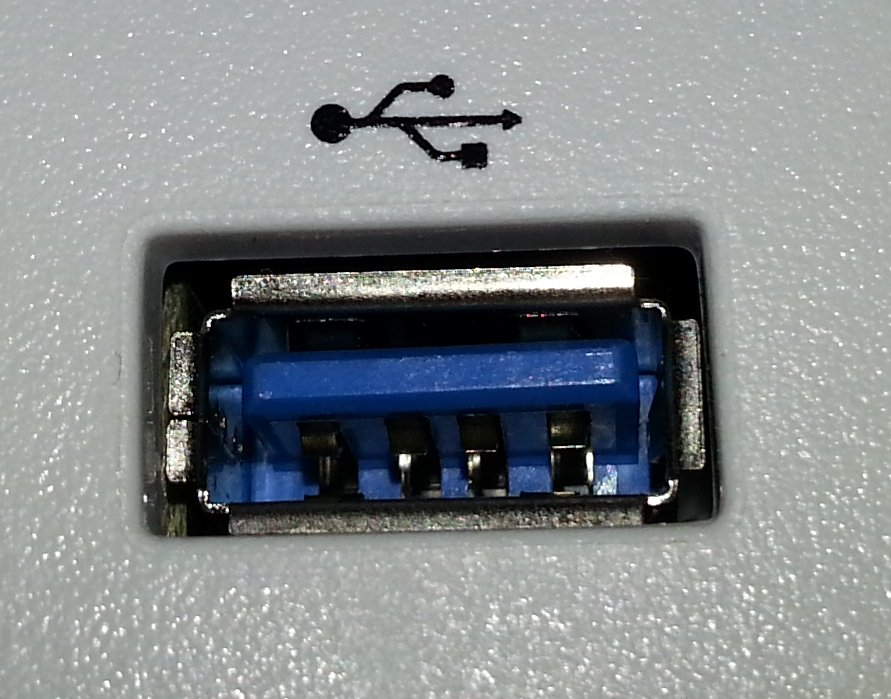
\includegraphics[width=8cm]{chapters/08-hw/img/usb-img.png}
	\caption{Port USB\protect\footnotemark}
	\label{fig:hw-usb}
\end{figure}

\footnotetext{\url{https://commons.wikimedia.org/wiki/File:Blue_USB_port_without_USB_3.0_contacts.jpg}
\textbf{CC0}}

Până în acest punct am discutat despre formele de conectare ale plăcilor de
extensie la unitatea de calcul. Plăcile de extensie au un element central de
aceeași importanță cu unitatea de procesare dintr-un sistem de calcul. Acel
element central poartă numele de \textit{chipset}. Chipset-ul implementează logica
centrală a dispozitivului, este cel care comunică cu sistemul de calcul. În
general driverele de care am discutat anterior, sunt dezvoltate pentru un anumit
chipset, și nu pentru o placă anume. Pot exista plăci de la mai mulți vendori,
care au același chipset. În acest caz același driver este compatibil și va fi
dezvoltat de producătorul chipset-ului, nu te integratorul plăcii. Dăm un
exemplu legat de o placă de rețea de 100 mbps cu chipset RTL8139 (Realtek este
producătorul chipset-ului): există cel puțin 2 producători (TP-Link și D-link)
pentru această placă. Plăcile arată diferit, au serii diferite, dar au același
chipset. Prin comparație putem lua două laptop-uri produse de HP și Dell care au
același procesor Intel. Aceste laptop-uri vor putea rula același sistem de
operare compatibil cu procesorul Intel fără nici o modificare. În încheierea
acestui paragraf am vrea să accentuăm faptul că o placa de extensie conține un
chipset care implementează logica necesară și de multe ori nu e suficient să
căutăm un vendor de renume, ci trebuie să ne uităm și la chipset de renume.

În continuare vom trece prin trei dintre cele mai importante plăci de extensie:
video, sunet, și rețea.

\subsection{Ce rol are placa video?}
\label{sec:hardware-extensii-gpu}

Placa video este o placă de extensie ce se conectează pe portul PCIe (în general
de tip x8 sau x16 pentru o viteză de comunicație ridicată) și are rolul de a
afișa pe monitor (ecran) elemente grafice. Pentru afișarea elementelor grafice,
în special în spațiu tri-dimensional, calcule complexe de geometrie trebuie
făcute. Pentru acest lucru, placa grafică este echipată cu unități specializate
de calcul matematic. Pe lângă unitățile de calcul, placa grafică mai dispune și
de propria memorie pentru a eficientiza timpul de procesare a datelor. La
achiziția unei plăci video (sau mai poartă denumirea de placă grafică - GPU
[\textit{Graphical Porcessing Unit}]) trebuie avute în vedere următoarele
aspecte: portul de conectare al plăcii (PCIe și la ce viteză), capacitatea
memoriei, frecvența de procesare, numărul de nuclee, precum și porturile de
ieșire. În \labelindexref{Figura}{fig:hw-gpu} sunt prezentate formatul
porturilor de ieșire ale unei plăci grafice: VGA, HDMI, DVI, DisplayPort. În
general plăcile grafice sunt produse cu o combinație între aceste porturi,
existând adaptoare la nevoie.

\begin{figure}[!htbp]
	\centering
	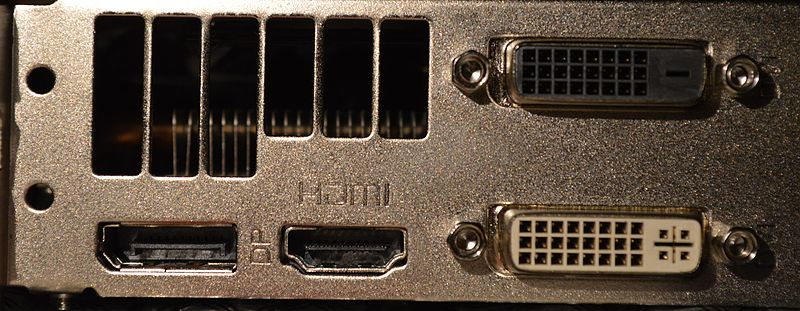
\includegraphics[width=8cm]{chapters/08-hw/img/gpu-img.png}
	\caption{Porturi ieșire placă grafică\protect\footnotemark}
	\label{fig:hw-gpu}
\end{figure}

\footnotetext{\url{https://commons.wikimedia.org/wiki/File:GPU_Interface.jpg}
\textbf{CC BY-SA 4.0}}

Atunci când veți analiza configurația unei plăci grafice, veți observa că
dispune de un număr foarte mare de nuclee (de ordinul zecilor/sutelor). Din
acest motiv, plăcile grafice (GPU-urile) sunt folosite și în prelucrarea de date
paralelă folosind framework-uri specifice (ex. OpenCL). De reținut că nucleele
prezente în placa grafică (GPU) nu se pot compara cu cele de pe unitatea de
procesare (CPU). Nucleele de pe GPU sunt optimizate să facă operații simple
aritmetice fără nici un fel de optimizare la verificări de condiție (branch-uri)
și predicție. GPU-ul nu poate înlocui rolul unui procesor.

\subsection{Ce rol are placa de sunet?}
\label{sec:hardware-extensii-audio}

Placa de sunet este o placă de extensie ce se poate conecta atât pe porturile
interne (PCI, PCIe), cât și pe cele externe (USB) și are rolul de a procesa
semnalele audio ce intră în calculator (microfoane) sau ies din calculator
(boxele). În esență placa de sunet conține un convertor digital-analogic prin
care convertește datele de pe calculator (digitale) în semnale analogice
(sunetul emis de boxe) și invers (de la analogic - captat de microfon - la
digital). În momentul în care achiziționați o placă de sunet trebuie să
inspectați următoarele caracteristici:

\begin{itemize}
	\item Puterea cu care poate emite (în general in Watt)
	\item Numărul de canale, implicit și numărul de porturi disponibile:
		cele mai des întâlnite sunt cele denumite 2.1 care au 2 boxe sau
		căști (stânga - dreapta) și cele denumite 5.1 care au 4 boxe (2
		spate stânga-dreapta, 2 față stânga -dreapta, 1 boxă centru)
	\item Modalitatea de conectare la calculator (internă pe PCI/PCIe sau
		externă pe USB)
\end{itemize}

În \labelindexref{Figura}{fig:hw-audio} este reprezentată o placă de sunet 5.1
ce se conectează pe portul intern PCI. Există câte un port de ieșire pentru
fiecare zonă (față, spate, centru), un port de intrare pentru microfon și un
port de intrare generic (pentru alte dispozitive).

\begin{figure}[!htbp]
	\centering
	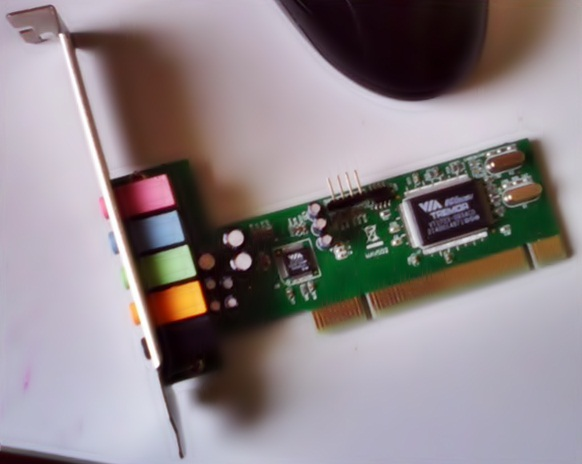
\includegraphics[width=8cm]{chapters/08-hw/img/audio-img.png}
	\caption{Placă de sunet\protect\footnotemark}
	\label{fig:hw-audio}
\end{figure}

\footnotetext{\url{https://commons.wikimedia.org/wiki/File:A_VIA_Envy_Sound_Card_5.1_6_Channels_(VIA_VT1617A).jpg}
\textbf{CC BY SA 4.0}}

\subsection{Ce rol are placa de rețea?}
\label{sec:hardware-extensii-net}

Placa de rețea este o placă de extensie cu ajutorul căreia un sistem de calcul
comunică la distanță cu alte sisteme de calcul. Prin intermediul plăcii de rețea
se primesc/trimit date necesare utilizatorului sistemului de calcul (ex. se
asigura accesul la Internet). Plăcile de rețea sunt de obicei interne
conectându-se pe porturile PCI, respectiv PCIe. Există și plăci de rețea externe
ce se pot conecta la portul USB dar de obicei acestea sunt mai lente.

La achiziția unei plăci de rețea trebuie ținut cont de următoarele caracteristici:

\begin{itemize}
	\item Portul pe care se conectează: este recomandat să fie PCIe dacă
		sistemul de calcul are un astfel de port disponibil. De asemenea
		trebuie verificată viteza portului PCIe (x1, x2, x4, x8, x16).
		În general se pot combina diferite viteze ale portului PCIe (fie
		că e vorba de placa de bază sau de placa auxiliară) iar viteza
		de funcționare va fi cea mai mică dintre cele 2
	\item Interfața disponibilă: în general cupru RJ-45 (protocol ethernet).
		Există și plăci cu suport de fibră optică: în descriere veți
		observa cuvântul cheie SFP \abbrev{SFP}{Small form-factor
		pluggable transceiver} (SFP+). Atenție pentru a utiliza suportul
		de fibră optică aveți nevoie de module speciale SFP ce au un
		cost mai ridicat decât cablul de cupru și de asemenea
		echipamentul în care vă conectați trebuie să suporte modul de
		fibră optică. În concluzie, în general veți alege portul de tip
		RJ-45.
	\item Viteza de transmisie: 100mbps, 1gbps, 10gbps. Cea mai răspândită
		în ziua de astăzi este viteza de 1Gbps.
\end{itemize}


Un lucru bun de menționat este acela că veți găsi diferențe foarte mari de preț
pentru o placă de rețea ce funcționează la viteza de 1Gbps. De exemplu o placă
de rețea Intel PCIe x1 pe 1Gbps poate ajunge la un pret de 400RON, în comparație
cu o placă de rețea TP-Link cu aceleași specificații care are un preț de
50-60RON. Motivul constă în eficiența chipset-ului plăcii: în cazul plăcii de
rețea Intel chipset-ul preia mare parte din funcția de procesare a datelor ce
vin/pleacă în comparație cu TP-Link unde procesarea este lăsată în grija
unității de procesare. Pentru o performanță sporită, mai ales în medii unde se
realizează transmisii de date cu volum ridicat, sunt recomandate plăcile de
rețea ce nu se bazează pe CPU atunci când trebuie să trimită/primească date.

% TODO: No license :(
%\begin{figure}[!htbp]
%	\centering
%	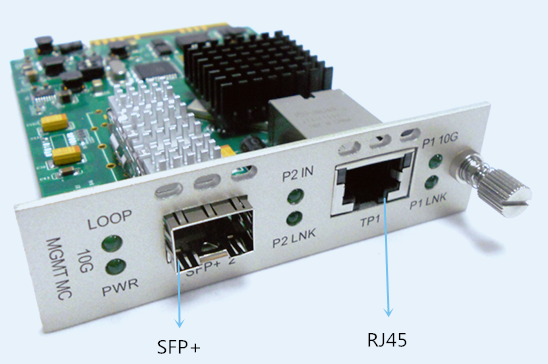
\includegraphics[width=8cm]{chapters/08-hw/img/net-img.png}
%	\caption{Placă de rețea cu port SFP+/RJ45}
%	\label{fig:hw-net}
%\end{figure}

\section{Facilități moderne în hardware}
\label{sec:hardware-functionalitati}

În mod curent producătorii de hardware încearcă să aducă noi facilități atât de
funcționalitate, cât și de securitate. Implementarea direct în hardware a
acestora aduce beneficiul performanței: execuția unei facilități în hardware
este mult mai rapidă decât alternativa execuției în software prin programe
dedicate. În cadrul acestei sencțiuni vom prezenta două facilități prezente în
hardware: Virtualizare și TPM \abbrev{TPM}{Trusted Platform Module}
(\textit{Trusted Platform Module}).

\subsection{Virtualizarea în hardware}
\label{sec:hardware-functionalitati-virt}

Pe un sistem de calcul putem rula un singur sistem de operare. Acesta trebuie să
aibă control total al componentelor sistemului și nu le poate partaja cu o altă
entitate. Acest lucru ne limitează la rularea unui singur sistem de operare la
un moment dat. O dată cu trecerea timpului, necesitatea rulării mai multor
tipuri de sisteme de operare, în același timp, pe același hardware, a crescut cu
scopul de a eficientiza anumite operații (testarea unor programe pe diverse
sisteme de operare) sau pentru a spori securitatea (un sistem de operare poate
oferi facilități de securitate suplimentare față de altul). Pentru a putea rula
mai multe sisteme de operare în același timp s-a introdus conceptul de
virtualizare (\textit{virtualization}): dacă se rulează mai multe sisteme de
operare în același timp, fiecare din ele va vedea o instanță virtuală a fiecărei
componente a sistemului (CPU virtual, memorie virtuală, disc virtual, etc). Se
realizează practic o multiplexare a fiecărei componente hardware. În anii
2005-2008 această multiplexare se realiza doar în software, fiind foarte lentă.
Din anii 2007-2009 s-a introdus conceptul de virtualizare în hardware, acesta
fiind suportat de către CPU. Viteza de rulare a sistemelor de operare
virtualizate a crescut, având aproape aceleași performanțe ca un sistem de
operare care rulează direct peste hardware. Pentru a beneficia de virtualizare,
aceasta trebuie activată din BIOS (vezi \labelindexref{Capitolul}{chapter:boot}).
De multe ori, fără activarea acestei opțiuni, soluțiile de virtualizare nu vor
funcționa indicând un mesaj de eroare corespunzător.

\subsection{Trusted Platform Module}
\label{sec:hardware-functionalitati-tpm}

Securitatea este un alt subiect dezbătut în piața IT\&C
\abbrev{IT\&C}{Information Technology and Communications}. Asigurarea
securității sistemelor a devenit o prioritate pentru fiecare companie din lume
(indiferent de domeniul de activitate). Instalarea de firewall-uri și antiviruși
este utilă pentru protecția atacurilor din exterior (din Internet), dar nu
protejează unitatea de calcul împotriva furtului fizic de date (ex.: daca un
laptop este furat, hoțul are acces la datele de pe laptop fără nici o problemă).
Pentru a preveni astfel de pierderi de date, unitățile de stocare ale
calculatoarele sunt criptate integral folosind algoritmi specifici. Pentru
criptare este necesară o cheie de criptare (asemănătoare unei parole). Această
cheie trebuie stocată într-un loc. În timp au fost întreprinse diverse metode de
stocare a cheilor (la începutul discului, pe un stick USB), dar nu au fost
suficiente. De aceea producătorii de procesoare au introdus un nou dispozitiv
numit TPM. TPM (\textit{Trusted Platform Module}) este un standard internațional
pentru un procesor criptografic capabil să stocheze chei criptografice (de
criptare). O dată criptat discul, cheile vor fi stocate în acesta și protejate
pe baza unei parole. Dacă unitatea de stocare va fi mutată pe alt calculator,
atacatorul nu va putea vedea datele. Doar modulul TPM ce stochează acele chei va
putea vizualiza conținutul unității de stocare. Modulul TPM trebuie activat din
BIOS, ca și virtualizare (vezi \labelindexref{Capitolul}{chapter:boot}).

\section{Abstractizarea dispozitivelor în Linux}
\label{sec:hardware-abstract-linux}

Pe calculatoarele ce rulează un sistem de operare bazat pe nucleul Linux,
dispozitivele sunt abstractizate (se văd) cu fișiere și se află în calea
absolută \file{/dev}. Dispozitivele din \file{/dev} sunt populate de către
framework-ul \texttt{udev} (Userspace \file{/dev}). Pe baza informațiilor
oferite de nucleu, acesta crează intrările puse la dipoziție utilizatorului in
\file{/dev}.

Fiind văzute ca fișiere, utilizatorul poate aplica aceleași operații pe care le
aplică fișierelor (vezi \labelindexref{Capitolul}{chapter:file-system}). Există
două tipuri de dispozitive în calea \file{/dev}:

\begin{itemize}
	\item Fizice - au un corespondent hardware
	\item Virtuale - nu au un corespondent hardware, sunt create de sistemul de operare.
\end{itemize}

Un exemplu de dispozitiv fizic este discul. Acesta este identificat printr-o intrare în sistemul de fișiere în directorul \file{/dev/}, intrare al cărei nume începe cu șirul \file{sd}
sau \file{hd} în funcție de inferfața de conectare. \labelindexref{Listing}{lst:hw:list-disks} prezintă rularea unei comenzi care afișează intrările din directorul \file{/dev/} corespunzătoare discurilor unui sistem.

\begin{screen}[caption={Afișarea intrărilor de tip disc},label={lst:hw:list-disks}]
[root@monitor ~]# ls -l /dev/sd*
brw-rw---- 1 root disk 8,  0 Jul  9 02:23 /dev/sda
brw-rw---- 1 root disk 8,  1 Jul  9 02:23 /dev/sda1
brw-rw---- 1 root disk 8,  2 Jul  9 02:23 /dev/sda2
brw-rw---- 1 root disk 8,  3 Jul  9 02:23 /dev/sda3
brw-rw---- 1 root disk 8, 16 Jul  9 02:23 /dev/sdb
brw-rw---- 1 root disk 8, 17 Jul  9 02:23 /dev/sdb1
\end{screen}

După cum se poate observa, avem 2 discuri (\file{sda} și \file{sdb}) fiecare cu
un număr diferit de partiții (vezi \labelindexref{Capitolul}{chapter:file-system}).
Asupra acestora putem executa aceleași operații ce se aplică și fișierelor. De exemplu, în \labelindexref{Listing}{lst:hw:disk-copy-bytes} sunt citiți primi 10 octeți de pe discul \file{sda}.

\begin{screen}[caption={Citirea datelor dintr-o intrare de tip disc},label={lst:hw:disk-copy-bytes}]
[root@monitor ~]# dd if=/dev/sda bs=1 count=10 -- | hexdump
0000000 48eb 1090 d08e 00bc b8b0
000000a
\end{screen}

Pe lângă dispozitivele fizice, în cadrul sistemului Linux, avem și dispozitive
virtuale cum ar fi:

\begin{itemize}
	\item \file{/dev/zero} - la citire generează zero-uri
	\item \file{/dev/random} - la citire generaza numere aleatorii
	\item \file{/dev/null} - la scriere, preia toate caracterele și le
		șterge (un coș de gunoi)
	\item \file{/dev/loop} - poate emula un disc ce este stocat într-un
		fișier (mai multe detalii în
		\labelindexref{Capitolul}{chapter:file-system})
\end{itemize}

Un exemplu de folosire a acestor dispozitive virtuale este prezentat în \labelindexref{Listing}{lst:hw:copy-dev-zero}. În acest exemplu sunt generate 10 octeți \texttt{0} într-un fișier. \textbf{Atenție!} Este vorba ca numărul \texttt{0} și nu de caracterul \texttt{0}; dacă am folosi comanda \cmd{cat} pe fișier, nu s-ar afișa nimic; de aceea am folosit
\cmd{hexdump}, pentru a vedea numerele codificate.

\begin{screen}[caption={Folosirea dispozitivelor virtuale},label={lst:hw:copy-dev-zero}]
[root@monitor ~]# dd if=/dev/zero of=test.zero bs=1 count=10
10+0 records in
10+0 records out
10 bytes (10 B) copied, 0.000491188 s, 20.4 kB/s
[root@monitor ~]# cat test.zero | hexdump
0000000 0000 0000 0000 0000 0000
[root@monitor ~]# dd if=/dev/zero of=test.zero bs=1 count=10 2> /dev/null
[root@monitor ~]#
\end{screen}

Dacă dorim să nu se mai afișeze informații despre cât a
scris comanda \cmd{dd} o putem redirecta către dispozitivul \file{/dev/null} ca în linia TODO din \labelindexref{Listing}{lst:hw:copy-dev-zero}.

\section{Anexă: Vizualizarea componentelor hardware pe Linux vs Windows}
\label{sec:hardware-virtualizare}

\subsection{Linux}
\label{sec:hardware-virtualizare-linux}

\begin{enumerate}
	\item Pentru a vizualiza dispozitivele descoperite la runtime de către
          nucleul Linux putem folosi comanda \cmd{dmesg}, ca în \labelindexref{Listing}{lst:hw:dmesg}.

\begin{screen}[caption={Afișarea mesajelor nucleului Linux (dmesg)},label={lst:hw:dmesg}]
Initializing cgroup subsys cpuset
Initializing cgroup subsys cpu
Linux version 2.6.32-573.8.1.el6.x86_64 (mockbuild@x86-ol6-builder-05) (gcc version 4.4.7 20120313 (Red Hat 4.4.7-16) (GCC) ) #1 SMP Tue Nov 10 02:36:19 PST 2015
Command line: ro root=UUID=ae064abe-b2fb-402b-8ba1-4ab1293bb584 rd_NO_LUKS rd_NO_LVM LANG=en_US.UTF-8 rd_NO_MD quiet SYSFONT=latarcyrheb-sun16 rhgb   KEYBOARDTYPE=pc KEYTABLE=us rd_NO_DM crashkernel=auto
KERNEL supported cpus:
  Intel GenuineIntel
  AMD AuthenticAMD
  Centaur CentaurHauls
BIOS-provided physical RAM map:
 BIOS-e820: 0000000000000000 - 000000000009d400 (usable)
 BIOS-e820: 000000000009d400 - 00000000000a0000 (reserved)
 BIOS-e820: 00000000000e0000 - 0000000000100000 (reserved)
 BIOS-e820: 0000000000100000 - 00000000d7fccf00 (usable)
 BIOS-e820: 00000000d7fccf00 - 00000000d7fd0000 (ACPI data)
 BIOS-e820: 00000000d7fd0000 - 00000000d8000000 (reserved)
 BIOS-e820: 00000000fec00000 - 0000000100000000 (reserved)
 BIOS-e820: 0000000100000000 - 00000001a8000000 (usable)
DMI 2.3 present.
SMBIOS version 2.3 @ 0xFDFE0
DMI: IBM eserver xSeries 336 -[883715Y]-/, BIOS -[APE128AUS-1.11]- 07/19/2005
e820 update range: 0000000000000000 - 0000000000001000 (usable) ==> (reserved)
e820 remove range: 00000000000a0000 - 0000000000100000 (usable)
No AGP bridge found
last_pfn = 0x1a8000 max_arch_pfn = 0x400000000
x86 PAT enabled: cpu 0, old 0x7040600070406, new 0x7010600070106
original variable MTRRs
reg 0, base: 0GB, range: 4GB, type WB
reg 1, base: 3456MB, range: 128MB, type UC
reg 2, base: 3584MB, range: 512MB, type UC
reg 3, base: 4GB, range: 4GB, type WB
total RAM covered: 7552M
Found optimal setting for mtrr clean up
\end{screen}


După cum se poate observa, după încărcare, nucleul a început cu inspectarea
zonelor de BIOS, după care a început enumerarea tuturor subcomponentelor din
sistemul de calcul.


	\item După pornirea sistemului, pentru a afișa informații despre
		hardware putem folosi comanda \cmd{lshw}, ce va afișa toate
		componentele sistemului sub formă arborescentă. Ieșirea comenzii
		este destul de stufoasă. O opțiune este folosirea parametrului
                \texttt{-short}, ce va face o sumarizare a configurației sistemului, ca în \labelindexref{Listing}{lst:hw:lshw}.

\begin{screen}[caption={Informații despre componentele hardware (lshw)},label={lst:hw:lshw}]
[root@monitor ~]# lshw -short
H/W path              Device       Class      Description
=========================================================
                                   system     eserver xSeries 336 -[883715Y]-
/0                                 bus        Motherboard
/0/0                               memory     60KiB BIOS
/0/4                               memory     16KiB L1 cache
/0/5                               memory     2MiB L2 cache
/0/8                               processor  Xeon
/0/9                               processor  CPU [empty]
/0/20                              memory     6GiB System Memory
/0/20/0                            memory     1GiB DIMM DDR Synchronous
/1                    eth1       network    Ethernet interface
\end{screen}

	\item Pentru a afișa doar componentele ce țin de interconectarea PCI,
          putem folosi comanda \cmd{lspci}, ca în \labelindexref{Listing}{lst:hw:lspci}.

\begin{screen}[caption={Informații despre componentele PCI (lspci)},label={lst:hw:lspci}]
[root@monitor ~]# lspci
00:00.0 Host bridge: Intel Corporation E7520 Memory Controller Hub (rev 0c)
00:00.1 Unassigned class [ff00]: Intel Corporation E7525/E7520 Error Reporting Registers (rev 0c)
00:02.0 PCI bridge: Intel Corporation E7525/E7520/E7320 PCI Express Port A (rev 0c)
00:04.0 PCI bridge: Intel Corporation E7525/E7520 PCI Express Port B (rev 0c)
00:06.0 PCI bridge: Intel Corporation E7520 PCI Express Port C (rev 0c)
00:07.0 PCI bridge: Intel Corporation E7520 PCI Express Port C1 (rev 0c)
00:08.0 System peripheral: Intel Corporation E7525/E7520/E7320 Extended Configuration Registers (rev 0c)
00:1d.0 USB controller: Intel Corporation 82801EB/ER (ICH5/ICH5R) USB UHCI Controller #1 (rev 02)
00:1d.1 USB controller: Intel Corporation 82801EB/ER (ICH5/ICH5R) USB UHCI Controller #2 (rev 02)
00:1d.7 USB controller: Intel Corporation 82801EB/ER (ICH5/ICH5R) USB2 EHCI Controller (rev 02)
00:1e.0 PCI bridge: Intel Corporation 82801 PCI Bridge (rev c2)
00:1f.0 ISA bridge: Intel Corporation 82801EB/ER (ICH5/ICH5R) LPC Interface Bridge (rev 02)
00:1f.2 IDE interface: Intel Corporation 82801EB (ICH5) SATA Controller (rev 02)
00:1f.3 SMBus: Intel Corporation 82801EB/ER (ICH5/ICH5R) SMBus Controller (rev 02)
01:01.0 VGA compatible controller: Advanced Micro Devices, Inc. [AMD/ATI] RV100 [Radeon 7000 / Radeon VE]
03:00.0 PCI bridge: Intel Corporation 6700PXH PCI Express-to-PCI Bridge A (rev 09)
03:00.2 PCI bridge: Intel Corporation 6700PXH PCI Express-to-PCI Bridge B (rev 09)
04:01.0 SCSI storage controller: LSI Logic / Symbios Logic 53c1030 PCI-X Fusion-MPT Dual Ultra320 SCSI (rev 08)
04:02.0 Ethernet controller: Intel Corporation 82545GM Gigabit Ethernet Controller (rev 04)
06:00.0 Ethernet controller: Broadcom Corporation NetXtreme BCM5721 Gigabit Ethernet PCI Express (rev 11)
07:00.0 Ethernet controller: Broadcom Corporation NetXtreme BCM5721 Gigabit Ethernet PCI Express (rev 11)
\end{screen}

	\item Pentru a afișa informații despre procesor putem interoga intrarea
		virtuală \file{/proc/cpuinfo} sau pentru o afișare mai sumarizată putem
                folosi comanda \cmd{lscpu}, ca în \labelindexref{lst:hw:lscpu}.

\begin{screen}[caption={Informații despre procesor},label={lst:hw:cpu}]
[root@monitor ~]# cat /proc/cpuinfo
processor       : 0
vendor_id       : GenuineIntel
cpu family      : 15
model           : 4
model name      : Intel(R) Xeon(TM) CPU 3.00GHz
stepping        : 3
microcode       : 5
cpu MHz         : 3000.000
cache size      : 2048 KB
physical id     : 0
siblings        : 2
core id         : 0
cpu cores       : 1
apicid          : 0
initial apicid  : 0
fpu             : yes
fpu_exception   : yes
cpuid level     : 5
wp              : yes
flags           : fpu vme de pse tsc msr pae mce cx8 apic mtrr pge mca cmov pat pse36 clflush dts acpi mmx fxsr sse sse2 ss ht tm pbe syscall lm constant_tsc pebs bts pni dtes64 monitor ds_cpl cid cx16 xtpr
bogomips        : 6000.14
clflush size    : 64
cache_alignment : 128
address sizes   : 36 bits physical, 48 bits virtual
power management:


[root@monitor ~]# lscpu
Architecture:          x86_64
CPU op-mode(s):        32-bit, 64-bit
Byte Order:            Little Endian
CPU(s):                2
On-line CPU(s) list:   0,1
Thread(s) per core:    2
Core(s) per socket:    1
Socket(s):             1
NUMA node(s):          1
Vendor ID:             GenuineIntel
CPU family:            15
Model:                 4
Stepping:              3
CPU MHz:               3000.000
BogoMIPS:              6000.14
L1d cache:             16K
L2 cache:              2048K
NUMA node0 CPU(s):     0,1
\end{screen}


	\item Pentru a afișa informații despre memorie putem interoga intrarea
		virtuală \file{/proc/meminfo} sau putem folosi comanda
                \cmd{free}, ca în \labelindexref{Listing}{lst:hw:memory}.

\begin{screen}[caption={Informații despre memorie},label={lst:hw:memory}]
[root@monitor ~]# free
             total       used       free     shared    buffers     cached
Mem:       5990840    5554088     436752          0     291060    2268304
-/+ buffers/cache:    2994724    2996116
Swap:      4194300      57328    4136972
[root@monitor ~]# cat /proc/meminfo
MemTotal:        5990840 kB
MemFree:          433932 kB
Buffers:          291060 kB
Cached:          2268376 kB
SwapCached:         2696 kB
Active:          2261704 kB
Inactive:        2878408 kB
Active(anon):    1591004 kB
Inactive(anon):   992200 kB
Active(file):     670700 kB
Inactive(file):  1886208 kB
Unevictable:           0 kB
Mlocked:               0 kB
SwapTotal:       4194300 kB
SwapFree:        4136972 kB
Dirty:               428 kB
Writeback:             0 kB
AnonPages:       2578592 kB
Mapped:            54352 kB
Shmem:              2528 kB
Slab:             307092 kB
SReclaimable:     268260 kB
SUnreclaim:        38832 kB
KernelStack:        4480 kB
PageTables:        24744 kB
NFS_Unstable:          0 kB
Bounce:                0 kB
WritebackTmp:          0 kB
CommitLimit:     7189720 kB
Committed_AS:    3409868 kB
VmallocTotal:   34359738367 kB
VmallocUsed:       34400 kB
VmallocChunk:   34359691292 kB
HardwareCorrupted:     0 kB
AnonHugePages:   2420736 kB
HugePages_Total:       0
HugePages_Free:        0
HugePages_Rsvd:        0
HugePages_Surp:        0
Hugepagesize:       2048 kB
DirectMap4k:        7984 kB
DirectMap2M:     6283264 kB
[root@monitor ~]# free
             total       used       free     shared    buffers     cached
Mem:       5990840    5557560     433280          0     291060    2268384
-/+ buffers/cache:    2998116    2992724
Swap:      4194300      57328    4136972
\end{screen}


	\item Pentru a monitoriza parametrii discului, putem folosi comanda
          \cmd{hdparm}, ca în \labelindexref{Listing}{lst:hw:disk}.

\begin{screen}[caption={Parametrii discului},label={lst:hw:disk}]
[root@monitor ~]# hdparm /dev/sda


/dev/sda:
SG_IO: bad/missing sense data, sb[]:  70 00 05 00 00 00 00 0a 00 00 00 00 20 00 00 00 00 00 00 00 00 00 00 00 00 00 00 00 00 00 00 00
 multcount     =  0 (off)
 readonly      =  0 (off)
 readahead     = 256 (on)
 geometry      = 8908/255/63, sectors = 143110144, start = 0
\end{screen}

\end{enumerate}

\subsection{Windows}
\label{sec:hardware-virtualizare-windows}

Pe sistemul de operare Windows pentru a vedea detalii despre componentele
atașate sistemului se poate folosi modulul \textit{Device Manager} (\texttt{Start -$>$ Run
-$>$ devmgmt.msc}).

\begin{figure}[!htbp]
	\centering
	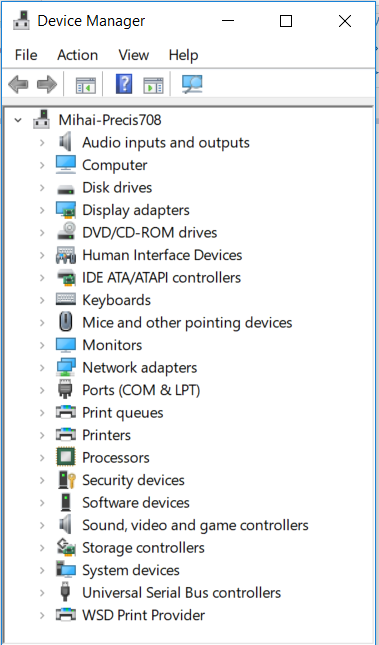
\includegraphics[width=6cm]{chapters/08-hw/img/devmanager-img.png}
	\caption{Device Manager}
	\label{fig:hw-devmanager}
\end{figure}

După cum se poate observa în \labelindexref{Figura}{fig:hw-devmanager}
componentele sunt grupate, dispuse arborescent (asemănător comenzii \cmd{lshw}
din Linux). Pentru a vedea ce dispozitive, respectiv modelul acestora, se
extinde grupul de interes. Pentru exemplu, vom extinde grupul
\textit{Processors}.

\begin{figure}[!htbp]
	\centering
	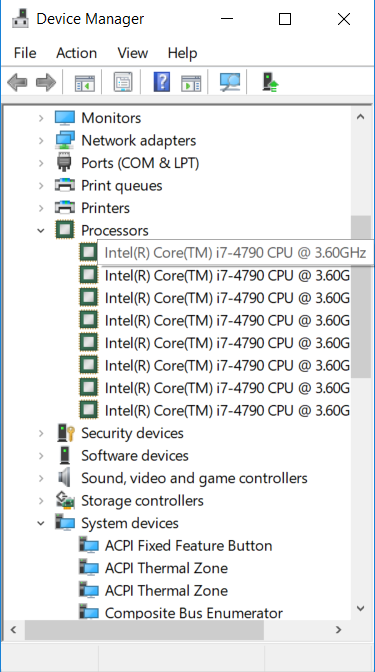
\includegraphics[width=6cm]{chapters/08-hw/img/devmanager-virt-img.png}
	\caption{Vizualizarea procesoarelor în Device Manager}
	\label{fig:hw-devmanager-virt}
\end{figure}


În \labelindexref{Figura}{fig:hw-devmanager-virt}, am extins secțiunea
\textit{Processors} și observăm 8 intrări întrucât avem 8 nuclee disponibile pe
sistemul acesta. Ne apare și varianta de procesor precum și frecvența acestuia
(i7-4790 la frecvența 3.6Ghz).

\section{Anexă: Vizualizarea versiunilor de drivere}
\label{sec:hardware-virtualizare-driver}

De-a lungul capitolului am subliniat importanța programelor ce rulează pe
sistemul de calcul și am accentuat modelul de dezvoltare al programelor, numite
drivere, care controlează componentele sistemului. Cele mai des întâlnite
probleme legate de stabilitatea unui sistem de calcul sunt cele cauzate de
dispozitivele atașate, respectiv driverele instalate pentru acestea. Este util
de știut cum vizualizăm ce drivere sunt active la un moment dat în sistem și
care e versiunea acestora.

\subsection{Vizualizarea driverele pe Linux}
\label{sec:hardware-virtualizare-linux}

Pe un sistem de operare cu nucleu Linux, vizualizarea driverelor se face cu
ajutorul comenzii \cmd{lsmod}, exemplificată în \labelindexref{Listing}{lst:hw:lsmod}.

\begin{screen}[caption={Vizualizarea modulelor / driverelor (lsmod)},label={lst:hw:lsmod}]
[root@monitor ~]# lsmod
Module                  Size  Used by
nfs                   431188  0
fscache                55636  1 nfs
nfsd                  311382  13
lockd                  73694  2 nfs,nfsd
nfs_acl                 2647  2 nfs,nfsd
auth_rpcgss            46084  2 nfs,nfsd
sunrpc                266331  18 nfs,nfsd,lockd,nfs_acl,auth_rpcgss
exportfs                4236  1 nfsd
\end{screen}


După cum se poate observa mai sus, comanda \cmd{lsmod} afișează doar driverele (sau
module în terminologia Linux), dimensiunea acestora în memorie și daca acestea
sunt folosite de alte drivere. Pentru a afla informații despre versiunea unui
driver/modul folosim comanda \cmd{modinfo}, ca în \labelindexref{Listing}{lst:hw:modinfo}.

\begin{screen}[caption={Informații despre un modul / driver (modinfo)},label={lst:hw:modinfo}]
[root@monitor ~]# modinfo nfs
filename:       /lib/modules/2.6.32-573.8.1.el6.x86_64/kernel/fs/nfs/nfs.ko
license:        GPL
author:         Olaf Kirch <okir@monad.swb.de>
srcversion:     154BF5D42DF2DCCEEC423E1
depends:        sunrpc,fscache,lockd,auth_rpcgss,nfs_acl
vermagic:       2.6.32-573.8.1.el6.x86_64 SMP mod_unload modversions
parm:           callback_tcpport:portnr
parm:           max_session_slots:Maximum number of outstanding NFSv4.1 requests the client will negotiate (ushort)
parm:           cache_getent:Path to the client cache upcall program (string)
parm:           cache_getent_timeout:Timeout (in seconds) after which the cache upcall is assumed to have failed (ulong)
parm:           recover_lost_locks:If the server reports that a lock might be lost, try to recover it risking data corruption. (bool)
parm:           enable_ino64:bool
parm:           nfs4_disable_idmapping:Turn off NFSv4 idmapping when using 'sec=sys' (bool)
parm:           dataserver_timeo:The time (in tenths of a second) the NFSv4.1  client  waits for a response from a  data server before it retries an NFS request. (uint)
parm:           dataserver_retrans:The  number of times the NFSv4.1 client retries a request before it attempts further  recovery  action. (uint)
\end{screen}

\cmd{modinfo} ne oferă informații despre locația fișierului pe disc, autorul
modului, ce dependențe are precum și versiunea (\texttt{vermagic}). Câmpul
\texttt{parm} descrie ce parametri poate primi acest modul la încărcare.

\subsection{Vizualizarea driverelor pe Windows}
\label{sec:hardware-virtualizare-windows}

În cadrul sistemului de operare Linux, informațiile despre drivere se pot afla
tot din \textit{Device Manager} (Start -> Run -> devmgmt.msc):

Pentru a vizualiza informații despre driverul procesorului, vom da click pe unul
din procesoarele listate în \labelindexref{Figura}{fig:hw-devmanager-virt}. Va
apărea o nouă fereastră ca în \labelindexref{Figura}{fig:hw-driver-virt} ce va avea
un tab denumit \textit{Driver}. Acesta ne va afișa toate informațiile relevant
despre driver:

\begin{itemize}
	\item Compania care a furnizat driverul (\textit{Driver Provider})
	\item Data la care a fost compilat (\textit{Driver Date})
	\item Versiunea (\textit{Driver Version})
	\item Semnătura (\textit{Digital Signer}) - în general driverele pe
		Windows trebuie semnate de un vendor agreat de Microsoft pentru
		a putea fi încărcate.
\end{itemize}

\begin{figure}[!htbp]
	\centering
	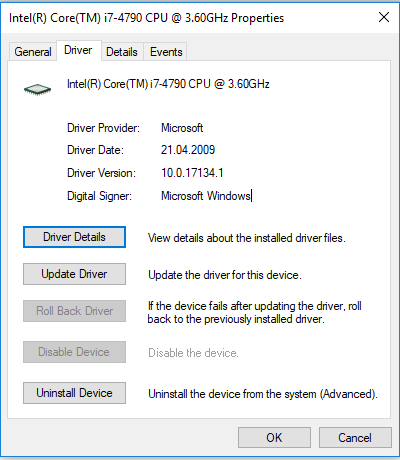
\includegraphics[width=8cm]{chapters/08-hw/img/driver-virt-img.png}
	\caption{Vizualizarea unui driver pe Windows}
	\label{fig:hw-driver-virt}
\end{figure}

\subsection{Vizualizarea componentelor pe Android}
\label{sec:hardware-virtualizare-android}

În mod implicit, în Android, nu există o opțiune prin care putem vizualiza
componentele hardware ale unui dispozitiv (telefon/tableta). Pentru acest lucru
putem folosi o aplicație ce poate fi instalată gratuit din PlayStore. O astfel
de aplicație este \textit{Android Hardware Info} (vezi
\labelindexref{Figura}{fig:hw-android})

\begin{figure}[!htbp]
	\centering
	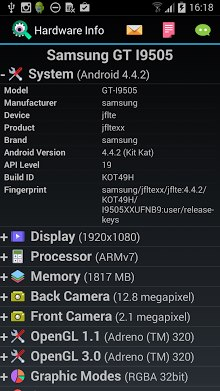
\includegraphics[width=8cm]{chapters/08-hw/img/android-img.png}
	\caption{Vizualizarea componentelor pe Android}
	\label{fig:hw-android}
\end{figure}
